\let\negmedspace\undefined
\let\negthickspace\undefined
\documentclass[journal,12pt,onecolumn]{IEEEtran}
\usepackage{cite}
\usepackage{amsmath,amssymb,amsfonts,amsthm}
\usepackage{algorithmic}
\usepackage{graphicx}
\graphicspath{{./figs/}}
\usepackage{textcomp}
\usepackage{xcolor}
\usepackage{txfonts}
\usepackage{listings}
\usepackage{enumitem}
\usepackage{mathtools}
\usepackage{gensymb}
\usepackage{comment}
\usepackage{caption}
\usepackage[breaklinks=true]{hyperref}
\usepackage{tkz-euclide} 
\usepackage{listings}
\usepackage{gvv}                                        
%\def\inputGnumericTable{}                                 
\usepackage[latin1]{inputenc}     
\usepackage{xparse}
\usepackage{color}                                            
\usepackage{array}
\usepackage{longtable}                                       
\usepackage{calc}                                             
\usepackage{multirow}
\usepackage{multicol}
\usepackage{hhline}                                           
\usepackage{ifthen}                                           
\usepackage{lscape}
\usepackage{tabularx}
\usepackage{array}
\usepackage{float}
\newtheorem{theorem}{Theorem}[section]
\newtheorem{problem}{Problem}
\newtheorem{proposition}{Proposition}[section]
\newtheorem{lemma}{Lemma}[section]
\newtheorem{corollary}[theorem]{Corollary}
\newtheorem{example}{Example}[section]
\newtheorem{definition}[problem]{Definition}
\newcommand{\BEQA}{\begin{eqnarray}}
\newcommand{\EEQA}{\end{eqnarray}}
\newcommand{\define}{\stackrel{\triangle}{=}}
\theoremstyle{remark}
\newtheorem{rem}{Remark}

\begin{document}

\title{2.9.7}
\author{ee25btech11056 - Suraj.N}
\maketitle
\renewcommand{\thefigure}{\theenumi}
\renewcommand{\thetable}{\theenumi}

\textbf{Question} :  

\begin{align*}
\vec{a}=2\hat{i}+\hat{j}+3\hat{k},\ \vec{b}=-\hat{i}+2\hat{j}+\hat{k},\ \vec{c}=3\hat{i}+\hat{j}+2\hat{k}
\end{align*}

\begin{center}
then find \(\vec{a}\cdot(\vec{b}\times\vec{c})\)
\end{center}

\begin{table}[h!]
  \centering
  

  \caption*{Table : vectors}
  \label{2.9.7}
\end{table}

\textbf{Solution} :

The Gram matrix \( \vec{G} \) for the vectors \( \vec{a}, \vec{b}, \vec{c} \) is:
\begin{align}
\vec{G} = \myvec{
\vec{a}^\top \vec{a} & \vec{a}^\top \vec{b} & \vec{a}^\top \vec{c} \\
\vec{b}^\top \vec{a} & \vec{b}^\top \vec{b} & \vec{b}^\top \vec{c} \\
\vec{c}^\top \vec{a} & \vec{c}^\top \vec{b} & \vec{c}^\top \vec{c}
}
\end{align}

Now, calculate the dot products:

\begin{align}
\vec{a}^\top \vec{a} = 2^2 + 1^2 + 3^2 = 4 + 1 + 9 = 14
\end{align}

\begin{align}
\vec{a}^\top \vec{b} = (2)(-1) + (1)(2) + (3)(1) = -2 + 2 + 3 = 3
\end{align}

\begin{align}
\vec{a}^\top \vec{c} = (2)(3) + (1)(1) + (3)(2) = 6 + 1 + 6 = 13
\end{align}

\begin{align}
\vec{b}^\top \vec{a} = \vec{a}^\top \vec{b} = 3
\end{align}

\begin{align}
\vec{b}^\top \vec{b} = (-1)^2 + 2^2 + 1^2 = 1 + 4 + 1 = 6
\end{align}

\begin{align}
\vec{b}^\top \vec{c} = (-1)(3) + (2)(1) + (1)(2) = -3 + 2 + 2 = 1
\end{align}

\begin{align}
\vec{c}^\top \vec{a} = \vec{a}^\top \vec{c} = 13
\end{align}

\begin{align}
\vec{c}^\top \vec{b} = \vec{b}^\top \vec{c} = 1
\end{align}

\begin{align}
\vec{c}^\top \vec{c} = 3^2 + 1^2 + 2^2 = 9 + 1 + 4 = 14
\end{align}

Thus, the Gram matrix \( \vec{G} \) is:
\begin{align}
\vec{G} = \myvec{
14 & 3 & 13 \\
3 & 6 & 1 \\
13 & 1 & 14
}
\end{align}

The characteristic equation is obtained by solving the determinant equation \( \mydet{\vec{G} - \lambda \vec{I}} = 0 \). The characteristic polynomial for the matrix is:

\begin{align}
\lambda^3 - 34\lambda^2 + 185\lambda - 100 = 0
\end{align}


To find the eigenvalues, we solve the cubic equation:
\[
\lambda^3 - 34\lambda^2 + 185\lambda - 100 = 0
\]
By solving this equation , we obtain the eigenvalues:
\begin{align}
\lambda_1 \approx 27.38, \quad \lambda_2 \approx 6.02, \quad \lambda_3 \approx 0.61.
\end{align}


The determinant of \( \vec{G} \) is the product of its eigenvalues:
\begin{align}
\mydet{\vec{G}} = \lambda_1 \lambda_2 \lambda_3 = 100.
\end{align}


The box product (scalar triple product) is the square root of the determinant of \( \vec{G} \):
\begin{align}
\vec{a} \cdot (\vec{b} \times \vec{c}) = \sqrt{\mydet{\vec{G}}} = \sqrt{100} = 10
\end{align}

As the three vectors form a left-handed system , the box product is negative. Hence, the negative value should be considered.

\textbf{Final Answer} : The value of \(\vec{a}\cdot(\vec{b}\times\vec{c})\) = -10
 
\pagebreak

\begin{figure}[h!]
  \centering
  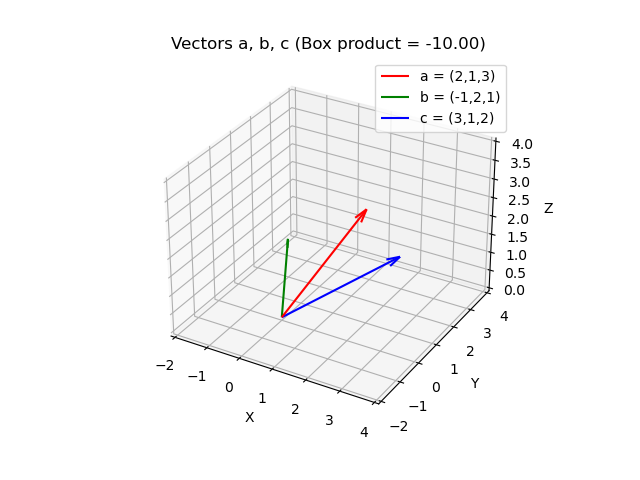
\includegraphics[width=0.7\columnwidth]{figs/vectors.png} 
   \caption*{Fig : Vectors}
  \label{Fig1}
\end{figure}



\end{document}
